
\documentclass[tikz,border=5pt]{standalone}
\usetikzlibrary{arrows.meta,positioning,calc,fit}

\begin{document}
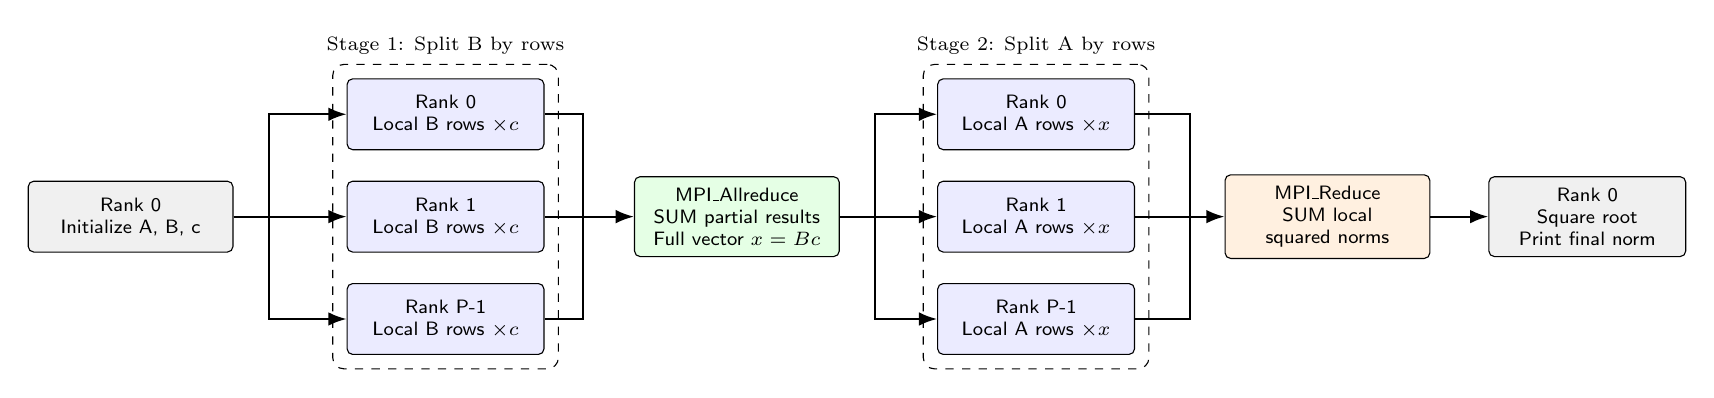
\begin{tikzpicture}[
        font=\sffamily\scriptsize,
        >=Latex,
        box/.style={
                draw,rounded corners=2pt,
                align=center,
                minimum height=9mm,
                inner sep=4pt
            },
        arr/.style={->,thick},
        rank/.style={
                box,fill=blue!8,
                minimum width=2.5cm
            }
    ]

    % Initialization
    \node[box,fill=gray!12,minimum width=2.6cm]
    (init) at (0,0)
    {Rank 0\\Initialize A, B, c};

    % Stage 1: B * c
    \node[rank] (b0) at (4,1.3)
    {Rank 0\\Local B rows $\times c$};

    \node[rank] (b1) at (4,0)
    {Rank 1\\Local B rows $\times c$};

    \node[rank] (bp) at (4,-1.3)
    {Rank P-1\\Local B rows $\times c$};

    % Distribute data
    \foreach \n in {b0,b1,bp}{
            \draw[arr] (init.east) -- ++(.45,0)
            |- (\n.west);
        }

    % Allreduce
    \node[box,fill=green!10,minimum width=2.6cm]
    (all) at (7.7,0)
    {MPI\_Allreduce\\SUM partial results\\Full vector $x=Bc$};

    % Stage 1 merging
    \coordinate (m1) at (5.75,0);
    \foreach \n in {b0,b1,bp}{
            \draw[thick] (\n.east) -- (5.75,0 |- \n.east)
            -- (m1);
        }
    \draw[arr] (m1) -- (all.west);

    % Stage 2: A * x
    \node[rank] (a0) at (11.5,1.3)
    {Rank 0\\Local A rows $\times x$};

    \node[rank] (a1) at (11.5,0)
    {Rank 1\\Local A rows $\times x$};

    \node[rank] (ap) at (11.5,-1.3)
    {Rank P-1\\Local A rows $\times x$};

    \foreach \n in {a0,a1,ap}{
            \draw[arr] (all.east) -- ++(.45,0)
            |- (\n.west);
        }

    % Reduce
    \node[box,fill=orange!12,minimum width=2.6cm]
    (reduce) at (15.2,0)
    {MPI\_Reduce\\SUM local\\squared norms};

    \coordinate (m2) at (13.45,0);
    \foreach \n in {a0,a1,ap}{
            \draw[thick] (\n.east) -- (13.45,0 |- \n.east)
            -- (m2);
        }
    \draw[arr] (m2) -- (reduce.west);

    % Final result
    \node[box,fill=gray!12,minimum width=2.5cm]
    (norm) at (18.5,0)
    {Rank 0\\Square root\\Print final norm};

    \draw[arr] (reduce.east) -- (norm.west);

    % Stage labels
    \node[draw,dashed,rounded corners,
        fit=(b0)(b1)(bp),
        inner sep=5pt,
        label={[font=\scriptsize]above:Stage 1: Split B by rows}
    ] {};

    \node[draw,dashed,rounded corners,
        fit=(a0)(a1)(ap),
        inner sep=5pt,
        label={[font=\scriptsize]above:Stage 2: Split A by rows}
    ] {};

\end{tikzpicture}
\end{document}
